\chapter{Informacje nieprawdziwe w dobie internetu}
Pojęcie ``Fake news'' odnosi się do 
informacji, które pomimo że nie posiadają pokrycia z rzeczywistością są 
przedstawiane jako prawdziwe w mediach takich jak np.: wiadomości, artykuły, 
portale społecznościowe itd.. 
Zwrot ten jest neologizmem i w języku angielskim oznacza dosłownie ``Fałszywe wiadomości''
celem wykorzystania takich wiadomości mogą być żarty np.: satyra, jednak najczęsciej 
mają one za zadanie oszukać odbiorce i wpłynąć na jego poglądy w sposób żądany przez autora
danej informacji. 

Fake news'y stały się bardzo popularnym zagadnieniem w ostatnich czasach ponieważ
internet a w szczególności media społecznościowe pozwoliły na przekazywanie 
informacji z niespotykaną wcześniej prędkością dzięki czemu rozprzestrzenianie 
dezinformacji stało się zadaniem stosunkowo prostym.

Zagadnienie to zyskało ogromny rozgłos podczas kampanii wyborczej oraz
prezydentury Donalda Trumpa, który zasłynął z częstego wykorzystywania 
tego zwrotu podczas wywiadów debat oraz wypowiedzi na mediach społecznościowych
tj. Twitter.
Do roku 2020 pojęcie ``Fake News'' zostało umieszczone w słownikach języka angielskiego
takich jak ``Oxford English Dictionary'', ``Macmillan Dictionary''.
\begin{figure}[h!]
    \centering
    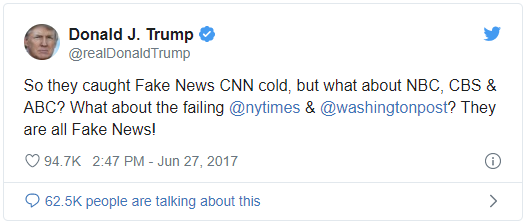
\includegraphics[width=0.7\textwidth]{./Img/Trump-Fake-News.png}
    \caption{Post udostępniony przez Donalda Trumpa na portalu Twitter}
\end{figure}

Według założonego przez dziewięć organizacji w skład których wchodzą 
Google, Facebook oraz Twitter projektu ``First Draft News''
możemy wyróżnić siedem typów Fake Newsów.
\begin{enumerate}
    \item Satyra bądź parodia
    \item Fałszywe połączenie
    \item Myląca zawartość
    \item Fałszywy kontekst
    \item Oszukana zawartość
    \item Zmanipulowana zawartość
    \item Sfabrykowana zawartość
\end{enumerate}
\section{Sposoby rozprzestrzeniania fałszywych informacji}

\section{Deep fake}

\section{Sposoby ochrony przed nieprawdziwymi informacjami}
